%%%% MoA Notes, these are still relevant



%%%%% MOA Section Old version
%%% FULL TABLE WITH ALL PHONEMES AND ALL VARIATIONS %%%%%%%%%
\iffalse
\begin{table}%[h]
\centering
\begin{tabular}{llp{0.5\linewidth}}
\toprule
\textbf{Language} & \textbf{ Phoneme Group} & \textbf{Phonemes} \\
\midrule
\multicolumn{3}{l}{\textbf{English}} \\
%Vowel & \textipa{i, iː, æ, ɐ, ɑ, ɑː, ɒ, ɒː, ə, ɚ, ɛ, ɝ, ɪ, ʉ, ʉː, ʊ} \\
%Vowel & \textipa{i, i:, {\ae}, 5, A, A:, 6, 6:, @, \textrhookschwa, E, \textrhookrevepsilon, \i, 0, 0:, U} \\ %% All 
& Vowel & \textipa{i, i:, {\ae}, 5, A, A:, 6, 6:, @, \textrhookschwa, E, \textrhookrevepsilon, \i, 0, 0:, U} \\
& Diphthong & \textipa{aj, aw, ej, ow, @w} \\
& Stop & \textipa{b, b\super j, c, c\super h, c\super w, d, d\super j, \|[{d}, k, k\super h, k\super w, p, p\super h, p\super j, p\super w, t, t\super h, t\super j, t\super w, \|[{t}, \textObardotlessj, \textObardotlessj\super w, g, g\super w, P} \\
& Nasal & \textipa{m, m \super j, \textsyllabic{m}, n, \textsyllabic{n}, N, M, \textltailn} \\
& Fricative & \textipa{f, f\super j, h, s, v, v\super j, z, \c{c}, D, S, Z, T} \\
& Affricate & \textipa{dZ, tS} \\
%Approximant & \textipa{j, l, w, ɫ, ɫ̩, ɹ, ʎ} \\
& Approximant & \textipa{j, l, w, \textltilde, \textsyllabic{\textltilde}, \*r, L} \\
& Closure & \textipa{sil} \\
%Tap \& Trill & \textipa{ɾ, ɾʲ, ɾ̃} \\
& Tap \& Trill & \textipa{R, R\super j, \~{R}} \\
\addlinespace
\multicolumn{3}{l}{\textbf{Spanish}} \\
& Vowel & \textipa{a, e, i, o, u} \\
& Stop & \textipa{b, c,  \|[{d}, k, p, \|[{t}, \textbardotlessj, \textbardotlessj J, g} \\
& Nasal & \textipa{m, n, N, M} \\
& Fricative & \textipa{f, s, x, \c{c}, D, G, S, J, B, T} \\
& Affricate & \textipa{tS} \\
& Approximant & \textipa{j, l, w, L} \\
& Closure & \textipa{sil} \\
& Tap \& Trill & \textipa{r, R} \\
\addlinespace
\multicolumn{3}{l}{\textbf{French}} \\
& Vowel & \textipa{a, e, i, o, u, y, \o, \ae, A, \~{A}, O, \~{O}, \textschwa, E, \~{E}} \\
& Stop & \textipa{b, c, d, k, p, t, \textObardotlessj, g} \\
& Nasal & \textipa{m, m\super j, n, N, \textltailn} \\
& Fricative & \textipa{f, s, v, z, K, S, Z} \\
& Affricate & \textipa{dZ, ts, tS} \\
& Approximant & \textipa{j, l, w, y, L} \\
& Closure & \textipa{sil} \\
\addlinespace
\multicolumn{3}{l}{\textbf{Polish}} \\
& Vowel & \textipa{a, i, u, O, \~{O}, E, \~{E}, 1} \\
& Stop & \textipa{b, b\super j, c, \|[{d}, k, p, p\super j, \|[{t}, t\super j, \textObardotlessj, g, P} \\
& Nasal & \textipa{m, m\super j, \|[{n}, N, \textltailn} \\
& Fricative & \textipa{f, f\super j, \|[{s}, v, v\super j, x, \|[{z}, \c{c}, C, \:s, \textcommatailz, \textctz} \\
& Affricate & \textipa{d\textcommatailz, d\textctz, \|[{d}\|[{z}, t\c{c}, t\:s, \|[{t}\|[{s}} \\
& Approximant & \textipa{j, \~{j}, l, w, L} \\
& Closure & \textipa{sil} \\
& Tap \& Trill & \textipa{r, r\super j} \\
\addlinespace
\bottomrule
\end{tabular}
\caption{Phonemes per language grouped by articulatory class. All of the available MFA tokens for all languages are used.}
\label{tab:phoneme_groups_by_language}
\end{table}
\fi
%%%%%%%%%%%%%%%%%%%%%%%%%%%%%%%%%%%%%%%%%%%%%%%%%%%%%%%%%%%%%%%%%%%%%%%%%%%%%

%%%%%%%%%%% change layout to phoneme groups being in a separate column to language
\iffalse
%\newpage
\begin{table}%[h]
\centering
\begin{tabular}{llp{0.5\linewidth}}
\toprule
\textbf{Language} & \textbf{Phoneme Group} & \textbf{Phonemes} \\
\midrule
\multicolumn{3}{l}{\textbf{English}} \\
%Vowel & \textipa{i, iː, æ, ɐ, ɑ, ɑː, ɒ, ɒː, ə, ɚ, ɛ, ɝ, ɪ, ʉ, ʉː, ʊ} \\
& Vowel & \textipa{i, {\ae}, 5, A, 6, @, E, \textrevepsilon, \i, u, U} \\
& Diphthong & \textipa{aj, aw, ej, ow, @w} \\
& Stop & \textipa{b, c, d, k, p, t, \j, g, P} \\
& Nasal & \textipa{m, n, N, M, \textltailn} \\
& Fricative & \textipa{f, h, s, v, z, c, D, S, Z, T} \\
& Affricate & \textipa{dZ, tS} \\
%Approximant & \textipa{j, l, w, ɫ, ɫ̩, ɹ, ʎ} \\
& Approximant & \textipa{j, l, w, \*r, L} \\
& Closure & \textipa{sil} \\
%Tap \& Trill & \textipa{ɾ, ɾʲ, ɾ̃} \\
& Tap \& Trill & \textipa{R} \\
\addlinespace
\multicolumn{3}{l}{\textbf{Spanish}} \\
& Vowel & \textipa{a, e, i, o, u} \\
& Stop & \textipa{b, c, k, p, \j, \j J, g} \\
& Nasal & \textipa{m, n, N, M} \\
& Fricative & \textipa{f, s, x, c, D, G, S, J, B, T} \\
& Affricate & \textipa{tS} \\
& Approximant & \textipa{j, l, w, L} \\
& Closure & \textipa{sil} \\
& Tap \& Trill & \textipa{r, R} \\
\addlinespace
\multicolumn{3}{l}{\textbf{French}} \\
& Vowel & \textipa{a, e, i, o, u, y, \o, \ae, A, O, \textschwa, E, \oe} \\
& Stop & \textipa{b, c, d, k, p, t, \j, g} \\
& Nasal & \textipa{m, n, N, \textltailn} \\
& Fricative & \textipa{f, s, v, z, K, S, Z} \\
& Affricate & \textipa{dZ, ts, tS} \\
& Approximant & \textipa{j, l, w, y, L, 4} \\
& Closure & \textipa{sil} \\
\addlinespace
\multicolumn{3}{l}{\textbf{Polish}} \\
& Vowel & \textipa{a, i, u, O, E} \\
& Stop & \textipa{b, c, d, k, p, t, \j, g, P} \\
& Nasal & \textipa{m, n, N, \textltailn} \\
& Fricative & \textipa{f, s, v, x, z, c, C, s} \\
%& Affricate & \textipa{dz, tc, ts} \\
& Affricate & \textipa{d\textcommatailz, d\textctz, t\c{c}, t\:s} \\
& Approximant & \textipa{j, l, w, L} \\
& Closure & \textipa{sil} \\
& Tap \& Trill & \textipa{r} \\
\addlinespace
\bottomrule
\end{tabular}
\caption{Phonemes per language grouped by articulatory class. This table lists one base symbol per MFA phoneme; a full inventory including all phonetic variants used in our experiments is given in Appendix~\ref{app_sec:chapter_5_appendix}, Table~\ref{app_tab:phoneme_groups_by_language}. \hl{THIS TABLE HAS BEEN MOVED TO EXPERIMENTAL DESIGN IT CAN PROBABLY BE REMOVED HERE}}
\fi


To further test this theory we can break down our phoneme data into sub-groups, this will allow us to explore whether the language or the phoneme groups are more important for recognition. Table \ref{ed_tab:phoneme_groups_by_language} shows the breakdown of phonemes in each phoneme group, the phonemes are selected from all of the phonemes in the MFA dictionaries for English and Spanish. All phonemes modifications, such as \textipa{a:} or \textipa{p\super j,}, are also included in the group with their unmodified phonemes. The full list of phoneme used in each language can be found in Appendix \ref{app_sec:chapter_5_appendix} Table \ref{app_tab:phoneme_class_acc_with_diff}.

The groups of phonemes chosen follow the same groupings as found in English et al. \cite{english2022domain} with some exceptions. All vowels were grouped together with any stessers also included. Diphthongs, that only exist in the English MFA dictionary, were separated into their own group, in order to test whether coarticulation between the phonemes may be relevant to the pretraining languages. Closure simply includes the "sil" token which denotes a lack of any sound for a short period of time. Finally the phonemes \textipa{r} and  \textipa{R} were separated into their own group, Tap \& Trill, while they could have been included in the Approximant group both \textipa{r} and \textipa{R} are much more frequent in the Spanish data so may be affected by pretraining data more than other approximants.

Figure \ref{ed_fig:Phonemes_Groups_English_linegraph} shows a breakdown of the average accuracy of different phoneme classes from the validation data from the English LibriSpeech dataset, the Multilingual LibriSpeech (MLS) Spanish subset, the MLS French subset and the MLS Polish dataset. The groups show accuracy from layer 7 of each of the 7 pretrained models for the nine different phoneme groups described in Table \ref{ed_fig:Phonemes_Groups_English_linegraph}. Figure \ref{ed_fig:Phonemes_Groups_English_barchart} shows the difference in accuracy of each phoneme group for each language when taken between the accuracy of the monolingual English model trained only on LibriSpeech data and the monolingual Spanish model trained only on the Multilingual LibriSpeech (MLS) Spanish subset as shown in equation \ref{ed_equ:CER_differrence_phoneme_groups}.

\begin{equation}\label{ed_equ:CER_differrence_phoneme_groups}
\centering
    CER\_on\_monolingual\_English - CER\_on\_monolingual\_Spanish
\end{equation}

In the vowel plot on Figure \ref{ed_fig:Phonemes_Groups_English_linegraph} we see that Spanish vowels have the highest accuracy across all models being above 80\% in all cases except the English monolingual model (960 / 0). Notably, Spanish has the fewest total individual vowels of all of the languages as seen in Table \ref{app_tab:phoneme_groups_by_language}, Spanish has no variants to the phonemes in the vowels which can occur less frequently in both training and validation data and therefore lower accuracy the average accuracy. It is also notable that the Polish vowels have the highest accuracy on the balanced mixed model (450 / 450), this could imply that when the testing language is unrelated to the pretaining languages individual phonemes are more impactful than the relationships between phonemes. Figure \ref{ed_fig:Phonemes_Groups_English_barchart} confirms that Polish vowels have the least difference between accuracy on each of the monolingual models, whilst English has the highest difference. 

Dipthongs were separated into a separate figure from vowels in order to evaluate whether language specific coarticulation affected accuracy, Dipthongs were only available in the English MFA dictionary. We see in \ref{ed_fig:Phonemes_Groups_English_linegraph} that English Dipthongs have higher accuracy on every model than their vowel counterparts, possibly due to the reduced set. English Dipthongs also have a higher difference between accuracy on monolingual models of 16.2\%. A full list of results for every model and the difference between the monolingual models can be found in Appendix \ref{app_sec:chapter_5_appendix}, Table \ref{app_tab:phoneme_class_acc_with_diff}.

For approximants in both Spanish and English the highest phoneme accuracy exists on their respective monolingual models. While the difference between models for Polish in Figure \ref{ed_fig:Phonemes_Groups_English_barchart} is in favour of the English monolingual model accuracy for Polish approximants is also high for the 800 / 100 model and the 300 / 600 model. French on the other hand has little difference between accuracy on either of the monolingual models and little variation for approximants across all models.

For nasals Figure \ref{ed_fig:Phonemes_Groups_English_barchart} shows all four languages having higher accuracy on the English monolingual model than on the Spanish monolingual model. Spanish has higher accuracy for nasal phonemes on the English monolingual when compared to the Spanish monolingual model, although it should be noted that Spanish nasals have the highest accuracy on the 100 / 800 model, so still a model with mostly Spanish training data. This may however show some nuance to the idea that all speech data benefits from monolingual or single domain pretraining. If a model is better at recognising phonemes from a a certain group this may be more beneficial for downstream recognition than simply pretraining on the same language. Since English, French and Polish also show higher accuracy on the English monolingual model this may support that theory. 

For the Tap \& Trill category Spanish has higher accuracy across all models when compared to both Polish and English and has 9.6\% more accuracy on the Spanish monolingual model when compared to the English monolingual mode. While in Figure  \ref{ed_fig:Phonemes_Groups_English_barchart} English has 15.3\% higher accuracy on the English monolingual model when compared to the Spanish monolingual model. However, on Figure \ref{ed_fig:Phonemes_Groups_English_linegraph} we can see that there is also an 11.8\% difference between the English monolingual model (960 / 0) and the model with balanced pretraining data (450 / 450), since the English accuracy for this group does not go above 33\% this suggests that recognition for phonemes in this group is not as dependant on the pretraining data as other groups. Similarly for Polish the average accuracy is low across all groups with the highest accuracy on the Spanish monolingual model at 21.4\%. While Polish does have higher accuracy on the Spanish monolingual model than on the English monolingual model it seems that phonemes in this group have low accuracy regardless of pretraining data. %\thoughts{do I need to come back to this when I know what's happening in the pretraining data?}

For Stops we see the pattern shown in previous sections with English phonemes having higher accuracy on the English monolingual model when compared to the Spanish monolingual model with a difference of 19.3\%. The Inverse is then true for Spanish, although to a lesser degree, with Spanish spoken phonemes having higher accuracy on the Spanish monolingual model and lower on the English model although this time with a difference of 1.3\%. Interestingly, the highest accuracy for Spanish is found on the balanced model (450 / 450), suggesting Spanish is benefitting from balanced monolingual pretraining in this category. French and Polish both have higher accuracy on the English monolingual model when compared to the Spanish monolingual model. This effect may be due to English having a larger variation of phonemes in this group when compared to Spanish, this may be beneficial for accuracy for phonemes in this group. French nasal phonemes have the highest accuracy across all models except the 300 / 600 model. 

For Affricates Polish shows the least variation with only 1.4\% difference between accuracy on the English and Spanish monolingual models. English has the highest accuracy on the English monolingual model and the lowest on the Spanish monolingual model showing preference to pretraining on the same language. Spanish however, has higher accuracy on the English monolingual model when compared to the Spanish monolingual model. The highest recorded accuracy is on the 450 / 450 model while the lowest is on the 300 / 600 model, giving Spanish the most variation of the languages in this category. As seen in Table \ref{app_tab:phoneme_groups_by_language} Spanish only contains one phoneme in this category, \textipa{tS}, and there are only 391 examples of the phoneme in the training data for the probes as seen in Table \ref{app_tab:phoneme_counts_per_language_train_10h_3}, when compared to phonemes that often have more than 10,000 examples. Training probes to recognise a single phoneme, with few examples may contribute to the variation in this case.

For Fricatives we see English again having higher accuracy on the English monolingual model when compared to the accuracy on the Spanish monolingual model. Spanish fricatives then have the highest accuracy on the Spanish monolingual model and the lowest on the English monolingual model. Both French and Polish have higher accuracy across all models than either English or Spanish, which is not true of any other phoneme group.

Finally for the closure group for French, Polish and English the accuracy on every model is higher than the accuracy in any other group for each model and for Spanish the only higher accuracy is found an all model except the English monolingual model in the vowel category. The closure category only contains the silence token (sil) given by the Montreal Forced Aligner when no sound is made. The high accuracy in Figure \ref{ed_fig:Phonemes_Groups_English_linegraph} across all languages and the lack of clear preference to either language in Figure \ref{ed_fig:Phonemes_Groups_English_barchart} suggests that silence is recognised accurately regardless of the model or the language the closure exists in.

Overall the findings in this section show that phoneme accuracy is not consistent across different categories of phonemes. As seen in nasals and affricates the concept that pretraining on the same or a related language always increases accuracy is not always true and in the case of Spanish stops and nasals, a balanced mix of pretraining can give the highest accuracy. In most cases however phonemes spoken in English do have higher accuracy on the models with the most English in pretraining and phonemes spoken in Spanish have the highest accuracy on the models with the most Spanish data in pretraining. 

For French, in all categories except closure phonemes in this language have higher accuracy recorded on the monolingual English model when compared to the monolingual Spanish model, which is consistent with the findings in Figure \ref{ed_fig:multilingual_barchart}. Accuracy is not consistent across all categories with a difference of 38\% between nasals and fricatives on the monolingual English model. For Polish, average accuracy is also inconsistent across categories, but is also less consistent across models with vowels having the highest accuracy on the 450 / 450 and approximants performing well on both the 800 / 100 model and the 300 / 600 model. 

These findings show that when the testing language is not in pretraining they do not necessarily benefit from monolingual training. 

%\thoughts{I feel that I need to expand this, I could possibly do this in the discussion section though}


%\newpage
\begin{figure}[H]
    %\centering
    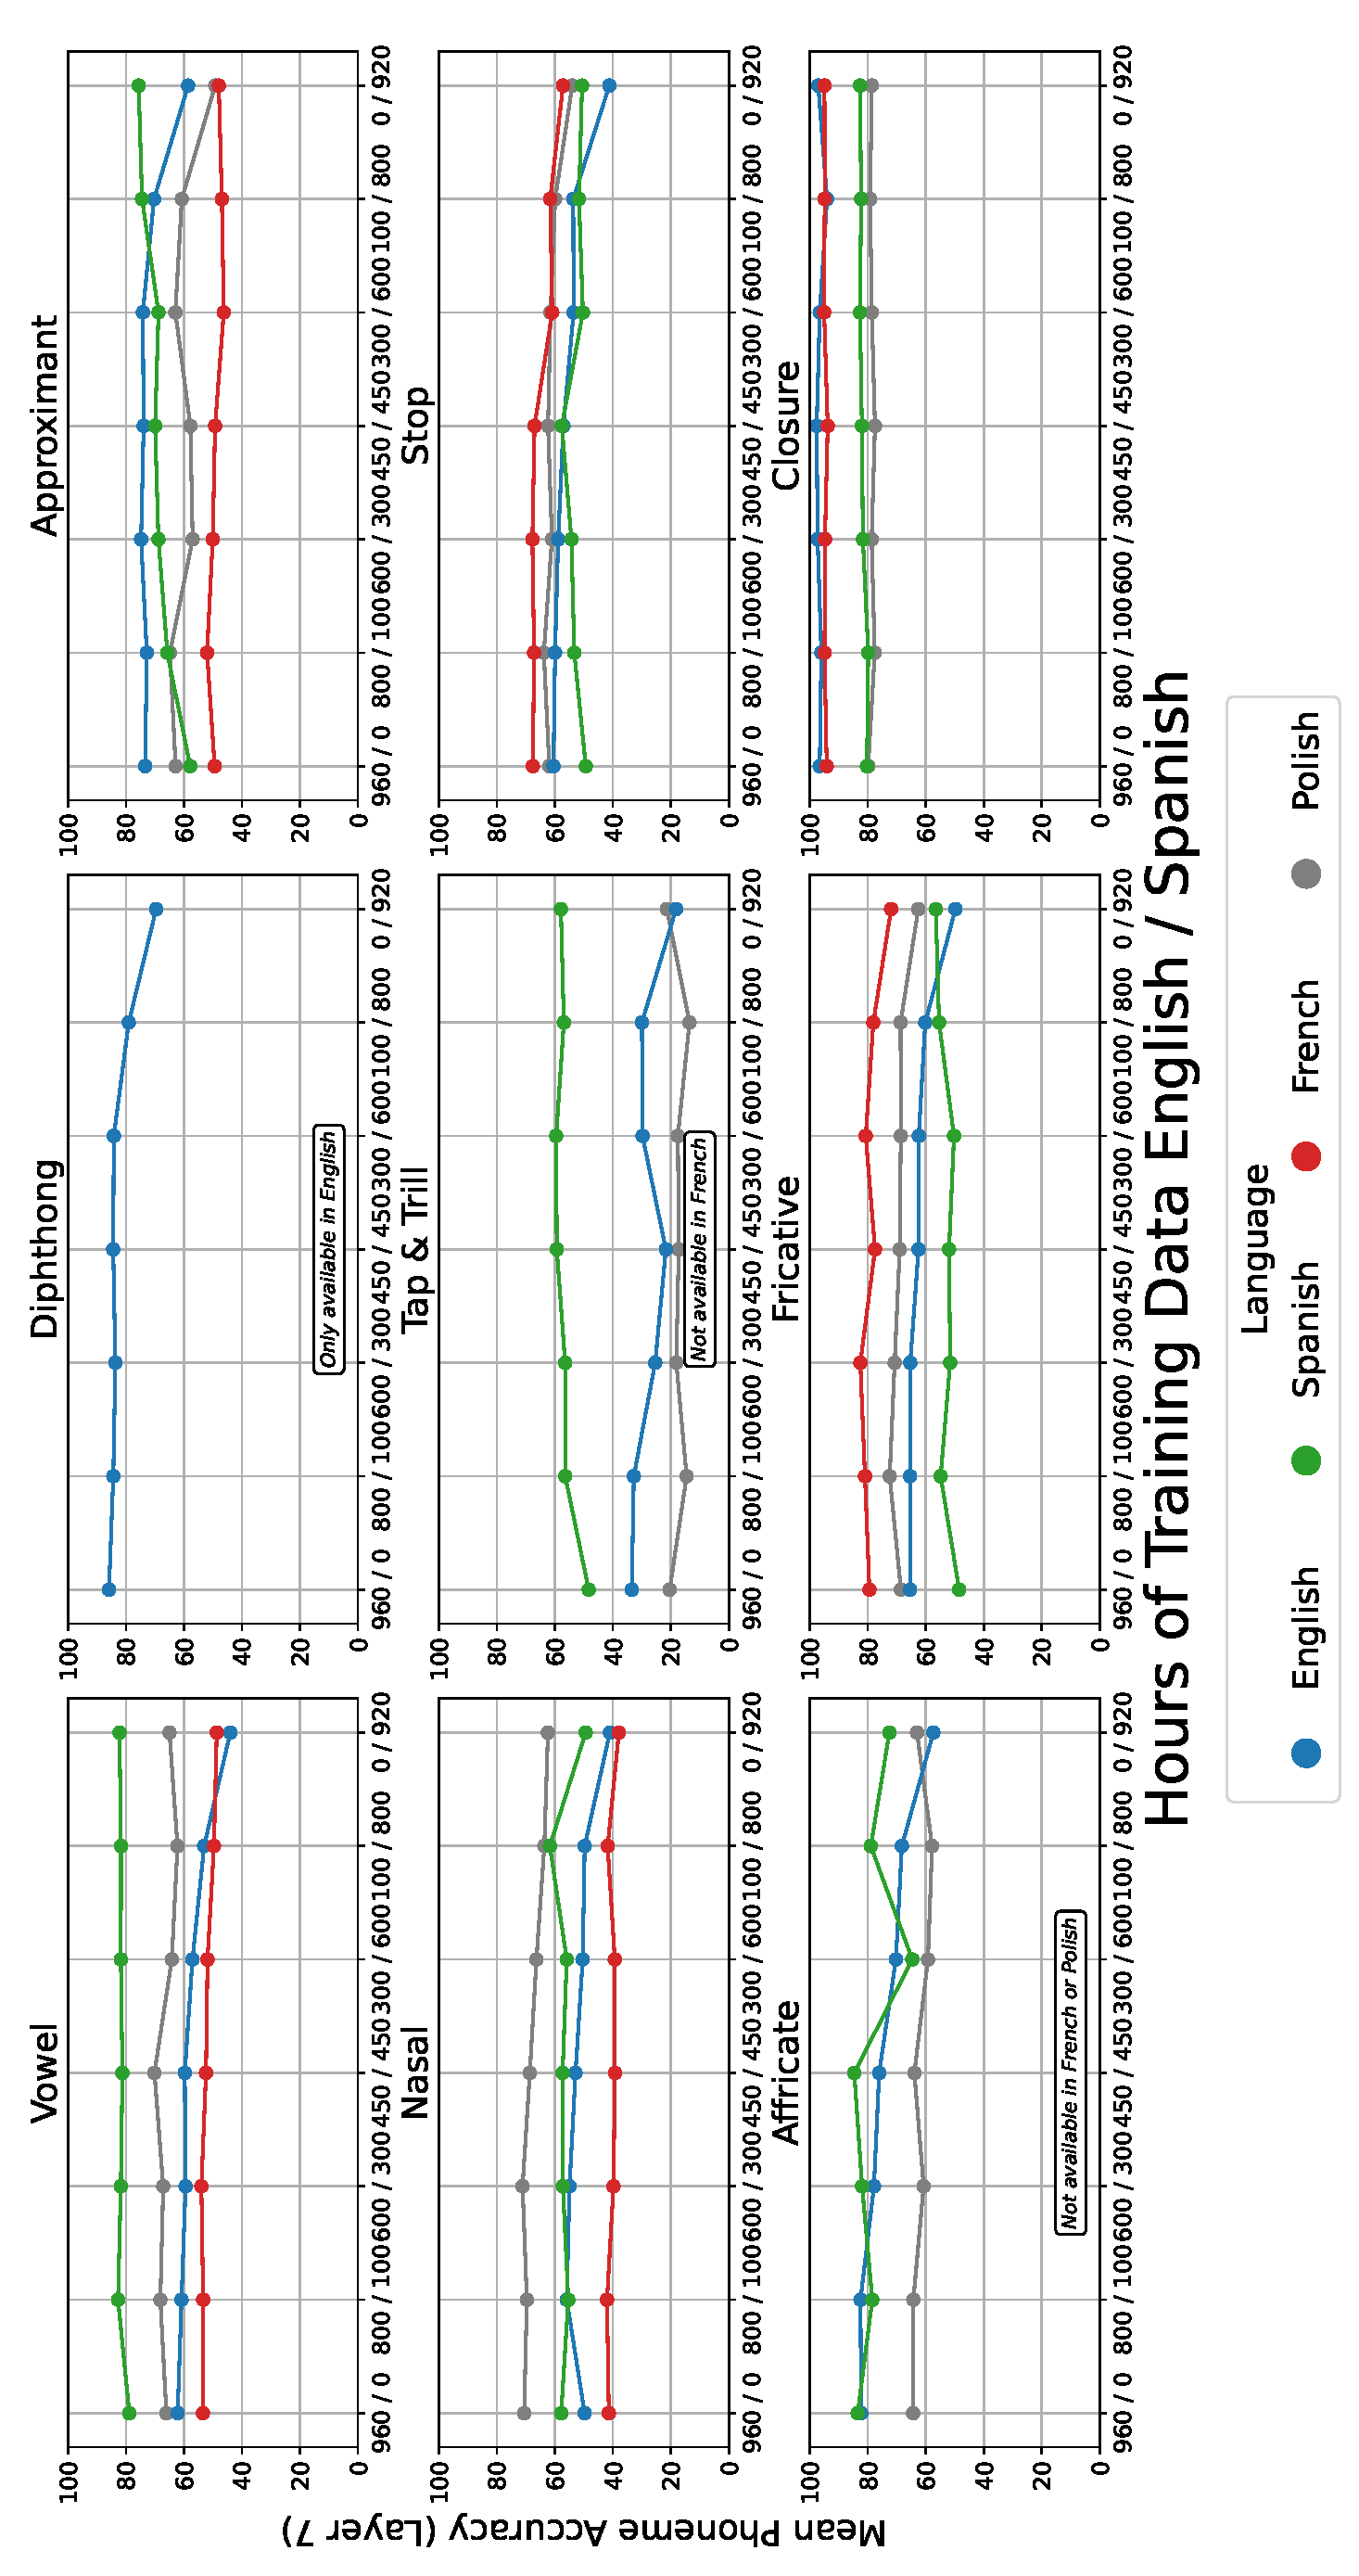
\includegraphics[height=0.9\textheight, width=0.75\paperwidth]{5_chapter5/figures/Rotate_phoneme_groups_line_graph_wpolish.pdf}
    \caption{Phoneme accuracy for 9 different phoneme groups. Accuracy is shown across all 7 pretrained models for four different languages: English, Spanish, French and Polish.}
    \label{ed_fig:Phonemes_Groups_English_linegraph}
\end{figure}

%\newpage
\begin{figure}[H]
    %\centering
    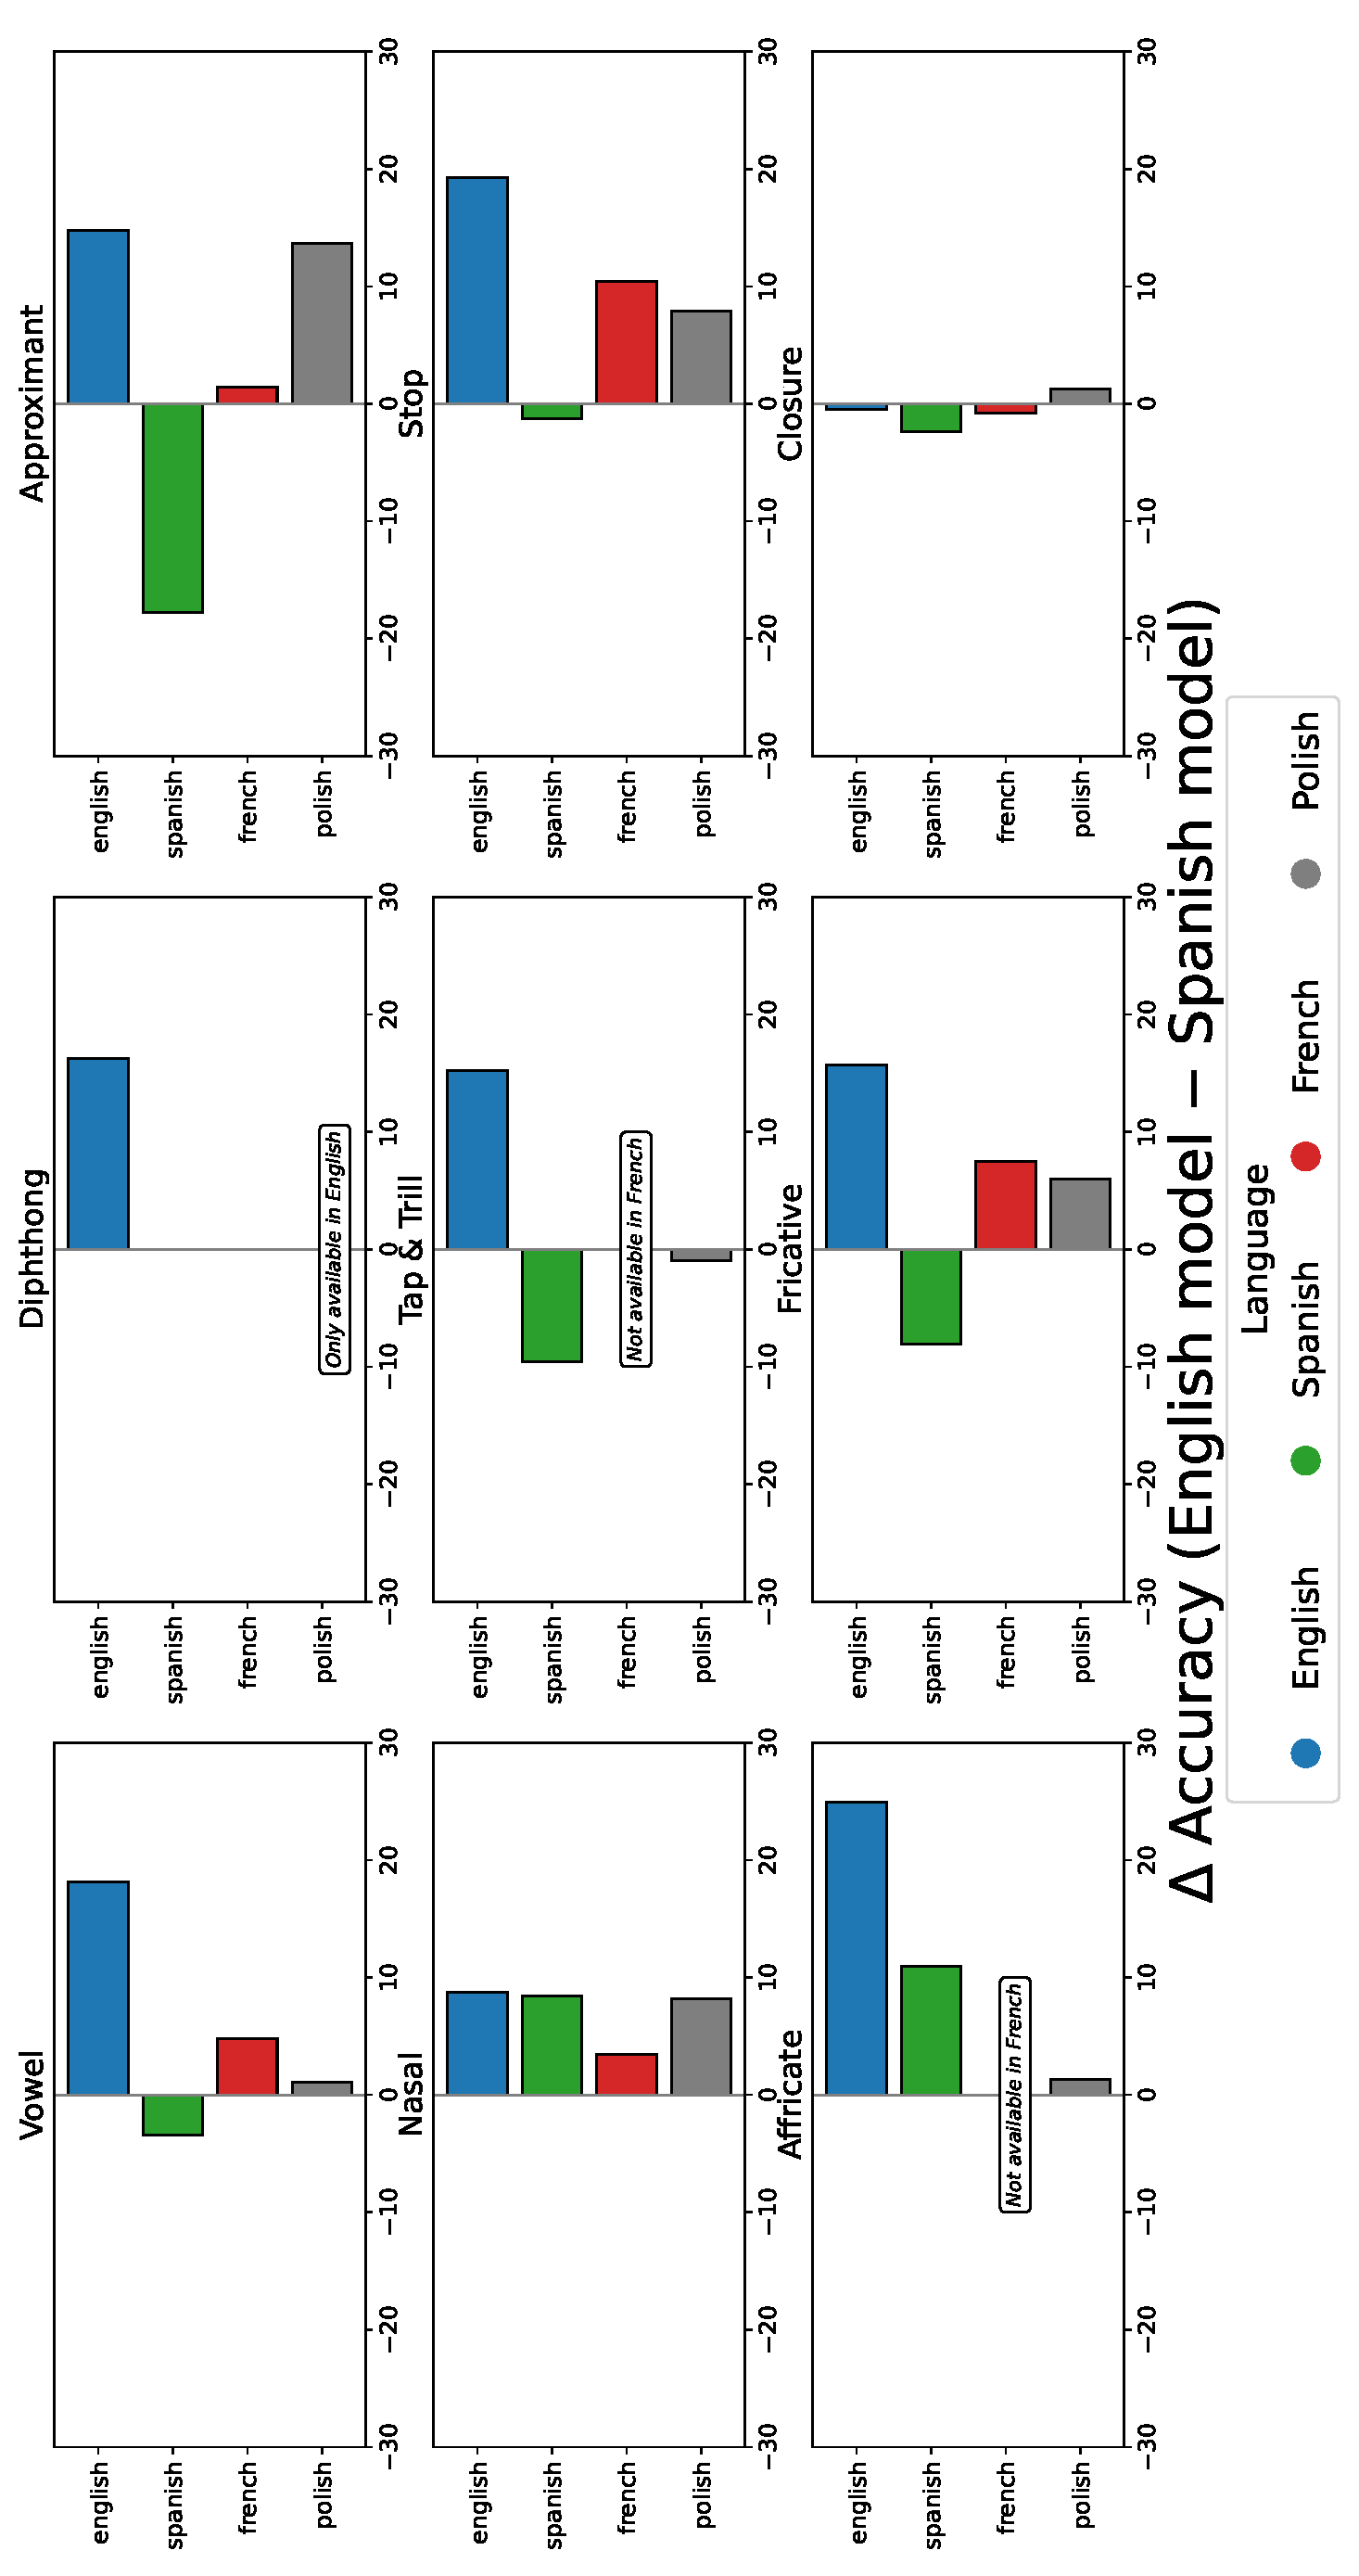
\includegraphics[height=0.9\textheight, width=0.75\paperwidth]{5_chapter5/figures/Rotate_phoneme_groups_bar_chart_wpolish.pdf}
    \caption{The difference between the accuracy of 9 different phoneme groups when measured between the English monolingual model and teh Spanish monolingual model. Accuracy is shown across all 7 pretrained models for four different languages: English, Spanish, French and Polish.}
    \label{ed_fig:Phonemes_Groups_English_barchart}
\end{figure}


%%%%%% Old Discussion

While phoneme accuracy and finetuned error rates may be better when language specific features are kept in the pretraining data the discovery that phoneme recognition can increase with language-agnostic training is important. 

For example, if a language, dialect or accent was very low-resource and did not have data from closely related languages in abundance SSL ASR could benefit from increasing the most common phonemes in said language by including data from unrelated languages. If we could design the pretraining data in this way we may be able to increase phoneme accuracy and lower error even for low-resource languages without having to resort to large models trained on large datasets. 

For future work, we would design a pretraining dataset that had the same phonetic makeup as a designated finetuning language. The pretraining data would include only data from languages unrelated to the one used in finetuning. We would expect such a model to achieve lower CER than a monolingual model trained on an unrelated language or a model trained on multilingual data that did not include the downstream language. 

Carefully designed pretraining data may even result in better performance than a model trained on multilingual data that contained small amounts of the finetuning language. This may be true as long as the finetuning target language was not the dominant language in pretraining, as per the behaviour exhibited by XLS-R in Chapter \ref{WC2}\info{previous chapter on pruning and bias}. These models could then all be compared to a monolingual model pretrained on a large dataset of the same language as finetuning, which we would expect to perform the best overall. 

If these experiments were successful we could have a simple method for increasing phoneme accuracy and CER for low-resource languages, dialects and accents. This method would only require the Montreal Forced Aligner and some knowledge of the target finetuning language to achieve.



%%%% Old Conclusion
Over the course of this chapter we have dissected how Self-Supervised Learning (SSL) Automatic Speech Recognition (ASR) models learn speech representations when pretrained with monolingual and multilingual training data. This gives us more insight into how SSL models learn and how we can leverage this knowledge for future work in this field. We started by pretraining 7 different versions of wav2vec 2.0 \cite{wav2vec} with different ratios of two different languages: English and Spanish. We pretrained 2 monolingual models, one on only English data from the LibriSpeech dataset \cite{librispeech} and one from only Spanish data from the Spanish subset of Multilingual LibriSpeech (MLS) \cite{MLS}. We then pretrained 5 more models with different ratios of the English and Spanish datasets.

We started in Section \ref{ed_subsec:same_data_finetuning} by fine-tuning to 100 hours subsets of LibriSpeech and MLS Spanish to observe the effect that our pretraining ratios had on finetuning results. We found that The English LibriSpeech data had the lowest Character Error Rate (CER) on the monolingual English model and the highest CER on the monolingual Spanish model with CER steadily increasing as the amount of English data was reduced in the pretraining data. For Spanish we found the inverse with Spanish data having the lowest CER on the monolingual Spanish model and the highest CER on the monolingual English model, with CER steadily increasing as the amount of Spanish data in pretraining was reduced.

In Section \ref{ed_subsec:gain_across_languages} we reproduced the results found in the previous section by testing the model with 10 hours of unseen English and Spanish data each from the FLEURs dataset \cite{FLEURS}. The same pattern was observed with the 10h English FLEURs dataset having the lowest CER on models with more English data in pretraining and Spanish. The 10h Spanish FLEURs shows the inverse pattern again by having the lowest CER on models with the most Spanish data and the highest CER on models with the least Spanish data. These experiments prove that pretraining on the same language as you are finetuning to gives the best results for ASR tasks.

In the same section we test multiple languages in the same languages families as English and Spanish, Germanic and Romance languages \cite{bauer2007linguistics}. We find that the Germanic languages Danish and German both have a positive difference towards English and the only language with a more positive difference than these languages is English. Similarly the Romance languages Asturian, Catalan and Italian have negative differences showing they perform better on the Spanish monolingual model when compared to the English monolingual model. French is an outlier among Romance languages showing a positive difference towards English. Finally we include 2 Slavic languages Polish and Russian, Polish shows a positive difference whereas Russian shows a negative difference. In this case Polish appears to benefit from English pretraining data and Russian benefits from Spanish Pretraining, which indicates that unrelated languages benefit much less from either pretraining languages. These findings confirm previous work that shows that pretraining on related languages can benefit downstream finetuning \cite{zhang2023fast, gupta2021clsril} however given that it has been shown that SSL ASR models learn phonetic characteristics and not semantic characteristics of speech \cite{pasad2021layer} it was important that we understand how the models are learning phonetic information when pretraining on multilingual data.

To understand how multilingual pretraining learns phoneme data we trained linear layer probes to recognise individual phonemes for each language. We collected the phoneme data using the Montreal Forced Aligner (MFA) and then created small 10 subsets of data from MLS to train the probes for phoneme recognition. In Section \ref{ed_sec:shared_vs_not_shared} after we test phoneme accuracy across all models for phonemes that exist in both English and Spanish data when compared to phonemes that are unique to either English or Spanish. Our findings show that the phonemes have the highest accuracy on the monolingual model trained on the same language they were spoken in, similar to the finetuning experiments in Section \ref{ed_subsec:gain_across_languages}. However, it is also notable that the English shared group has higher accuracy than the English Unique group across all models. It was also true that the Spanish Shared group had higher accuracy on every model when compared to the Spanish Unique group. 

This suggested that phonemes will have higher accuracy if there are more examples of it in pretraining even if those examples are spoken in different languages. We test this by introducing phoneme data collected from 2 new 10 hour subsets of MLS: MLS French and MLS Polish. These languages were chosen because French had outlier behaviour in Figure \ref{ed_fig:multilingual_barchart} and Polish is a Slavic language unrelated to English or Spanish. We split the phoneme accuracy data into groups, phonemes shared by English and Spanish spoken in each language and phonemes unique to French or Polish. The results showed that phonemes that are found in both English and Spanish always perform better than phonemes that are unique to either French or Polish even when the shared phonemes were spoken in French or Polish. This suggests that even when a phoneme is spoken in a language unrelated to either of the pretraining languages accuracy can be higher if the model has seen it in pretraining.

In Section \ref{ed_sec:phonemes_classes} we explored whether phoneme group accuracy trends across multilingual pretrained models behaved differently when spoken in 4 different languages: English, Spanish, French and Polish. We found that for English and Spanish in most cases phonemes would perform better when tested on a model with more data from their native language. The exceptions being Affricates where the models with the most English have the highest accuracy, however only one phoneme exists in the affricate class in Spanish and there are much less examples in the training data for Spanish. French and Polish phonemes were more likely to perform better on the models trained with more English data, with some exceptions. For Polish performance for the Tap \& Trill group was marginally higher for models with more Spanish data, which may be due to Spanish having more examples of the phonemes in this group in the pretraining set. 

Finally with the knowledge learned throughout this chapter we suggest future work that could be undertaken. We suggest that error rates on low-resource languages could be reduced by using data from languages that do not have to have any relation to the target finetuning language. A pretraining dataset could created using any languages as long and an appropriate number of all of the relevant phonemes in your target language were included in pretraining.

The consistent themes that emerged from this chapter were that SSL ASR benefits from pretraining on the same or related languages to the finetuning language and that this is true for phoneme recognition as well. The secondary theme is that when there are more training examples for an individual phoneme, accuracy can be increased on that phoneme, regardless of language specific interactions such as coarticulation. Overall, it has been seen throughout the chapter that selecting your pretraining data with care can be a great benefit in ASR and that there is more to SSL ASR than just the language relationships between your pretraining and finetuning languages.
